\section{Model}

This section describes our model. We will start by describing a simplistic
version of our model, and continue to introduce new properties until we reach
the full model.

\newcommand{\CostPerChunk}{\ensuremath{\textsc{cost}}}
\newcommand{\Distance}{\ensuremath{\textsc{dist}}}

\subsection{Symbols}

This is a dummy section to introduce the symbols used later...

\begin{description}
 \item [$\Tree$] the substrate tree with $\Tree = (\SubstrateNodes , \SubstrateEdges)$
 \item [$\SubstrateNodes$]  a set of nodes: $\{\SubstrateNode_1, \dots ,
\SubstrateNode_{|\SubstrateNodes|}\}$
 \item [$\SubstrateEdges$] a set of edges : $\{\SubstrateEdge_1, \dots ,
 \SubstrateEdge_{|\SubstrateEdge|}\}$ with $\SubstrateEdge_1 =
(\SubstrateNode_i, \SubstrateNode_j)$
 \item [$c_i$] A chunk of type $i$
 \item [$v_i$] The i-th $\VM$ of the request
 \item [$\VirtualNodes$] the set of virtual Nodes = $\{1,2,\dots,\VCSwitch\}$
 \item [$\VirtualEdges$] the set of virtual Edges, $e_{V1}$ connects $1 \in
\VirtualNodes$ with $\VCSwitch \in \VirtualNodes$.
 \item [$\hat f$] the maximal flow
 \item [$|\hat f|$] the value of the maximal flow


 \item [$\Bandwidth$] Bandwidth constraint of an edge
 \item [$\CostTrans$] cost of chunk transport
 \item [$\CostCom$] cost of chunk communication
 \item [$\Vms$] number of VMs to spawn
 \item [$\ChunkTypes$] number of chunk types placed in an instance
 \item [$\Formula$] a formula
 \item [$\Clauses$] set of clauses in a formula
 \item [$\NClauses$] number of clauses in a given formula
 \item [$\Vars$] set of variables in a given formula
 \item [$\NVars$] number of variables in a given formula
 \item [$\Thr$] threshold
 \item [$\VCB$] virtual cluster model with bandwith
 \item [$\VCNB$] virtual cluster model without bandwith
 \item [$\varx$] variable
 \item [$\positive$] positive subtree of a gadget
 \item [$\negative$] negative subtree of a gadget
 \item [$\SAT$] set of satisfiable boolean formulas in CNF
 \item [$\TSAT$] set of satisfiable boolean formulas in 3CNF
 \item [$\Val$] valuation
 \item [$\Sol$] soultion to VC instance

\end{description}



\subsection{The Basic Model}

\carlo{Section TODO: How many / which figures + order?}

In the basic version of $\Problem$ data in the form of multiple chunks is
located in an undirected host graph tree $\Tree = (\SubstrateNodes,
\SubstrateEdges)$. A chunk $\Chunk$ of the set of chunks $\Chunks =
\{\Chunk_1,\dots,\Chunk_{\ChunkTypes}\}$ can only be located at the leaves
$\Leaves = \{\Leaf_1,\dots,\Leaf_m\} \subset \SubstrateNodes$ of $\Tree$. We
denote the location of a chunk by $\ChunkLocation : \Chunks \rightarrow
\Leaves$. A cluster, consisting of a set of VMs $\VirtualNodes =
\{\VirtualNode_1,\dots,\VirtualNode_{\Vms}\}$, is allready embedded on the host
graph, and should process this data. The VMs are embedded on the
leaves of the tree, and we denote the location of the VMs by $\NodeMapping :
\VirtualNodes \rightarrow \Leaves$. We assume that $\Vms = \ChunkTypes$, each
VM $\VirtualNode_i$ can read the data of one chunk $\Chunk_j$, and the data of
each chunk $\Chunk_j \in \Chunks$ has to be processed. In order to process the
data from a chunk $\Chunk_j$ with the VM $\VirtualNode_i$ it has to be
transferred along a (potentially empty) path $\Path_j =
\{\SubstrateEdge_{j_1},\dots,\SubstrateEdge_{j_n}\} ~ \SubstrateEdge_{j_k} \in
\SubstrateEdges$ such that $\SubstrateEdge_{j_1} = (\ChunkLocation(\Chunk_j),
\SubstrateNode_x)$, $\SubstrateEdge_{j_k} = (\SubstrateNode_x,
\SubstrateNode_y) \rightarrow \SubstrateEdge_{j_{k+1}} = (\SubstrateNode_y ,
\SubstrateNode_z)$, and $\SubstrateEdge_n = (\SubstrateNode_y,
\NodeMapping(\VirtualNode_i))$.  For the sake of simplicity we assume that
transferring a chunk over a link in the host graph inflicts bandwidth cost of
$\CostTrans$ on this link. \carlo{NEW: We refer to the sum of all bandwidth 
costs for the transport of specific chunks to vms by the function 
$\CostPerChunk : \Chunks \cup \VirtualNodes \rightarrow \mathbb{R}$. Note, that 
$\CostPerChunk(\Chunk_j) = \CostPerChunk(\VmChunkAssignment(\Chunk_j))$ and
$\CostPerChunk(\Chunk_j) = \Distance(\ChunkLocation(\Chunk_j), 
\NodeMapping(\VmChunkAssignment(\Chunk_j))) \cdot \CostTrans$, where $\Distance 
: \SubstrateNodes \times \SubstrateNodes \rightarrow \mathbb{N}$ denotes the 
distance in number of hops of two nodes in the host graph.} The overall 
objective of $\Problem$ is to find an
assignment of VMs to chunks $\VmChunkAssignment : \Chunks \rightarrow
\SubstrateNodes$, so that the overall costs $\sum_{j \in
\{1,\dots,\ChunkTypes\}} |\Path_j|$ are minimized.

\begin{figure}

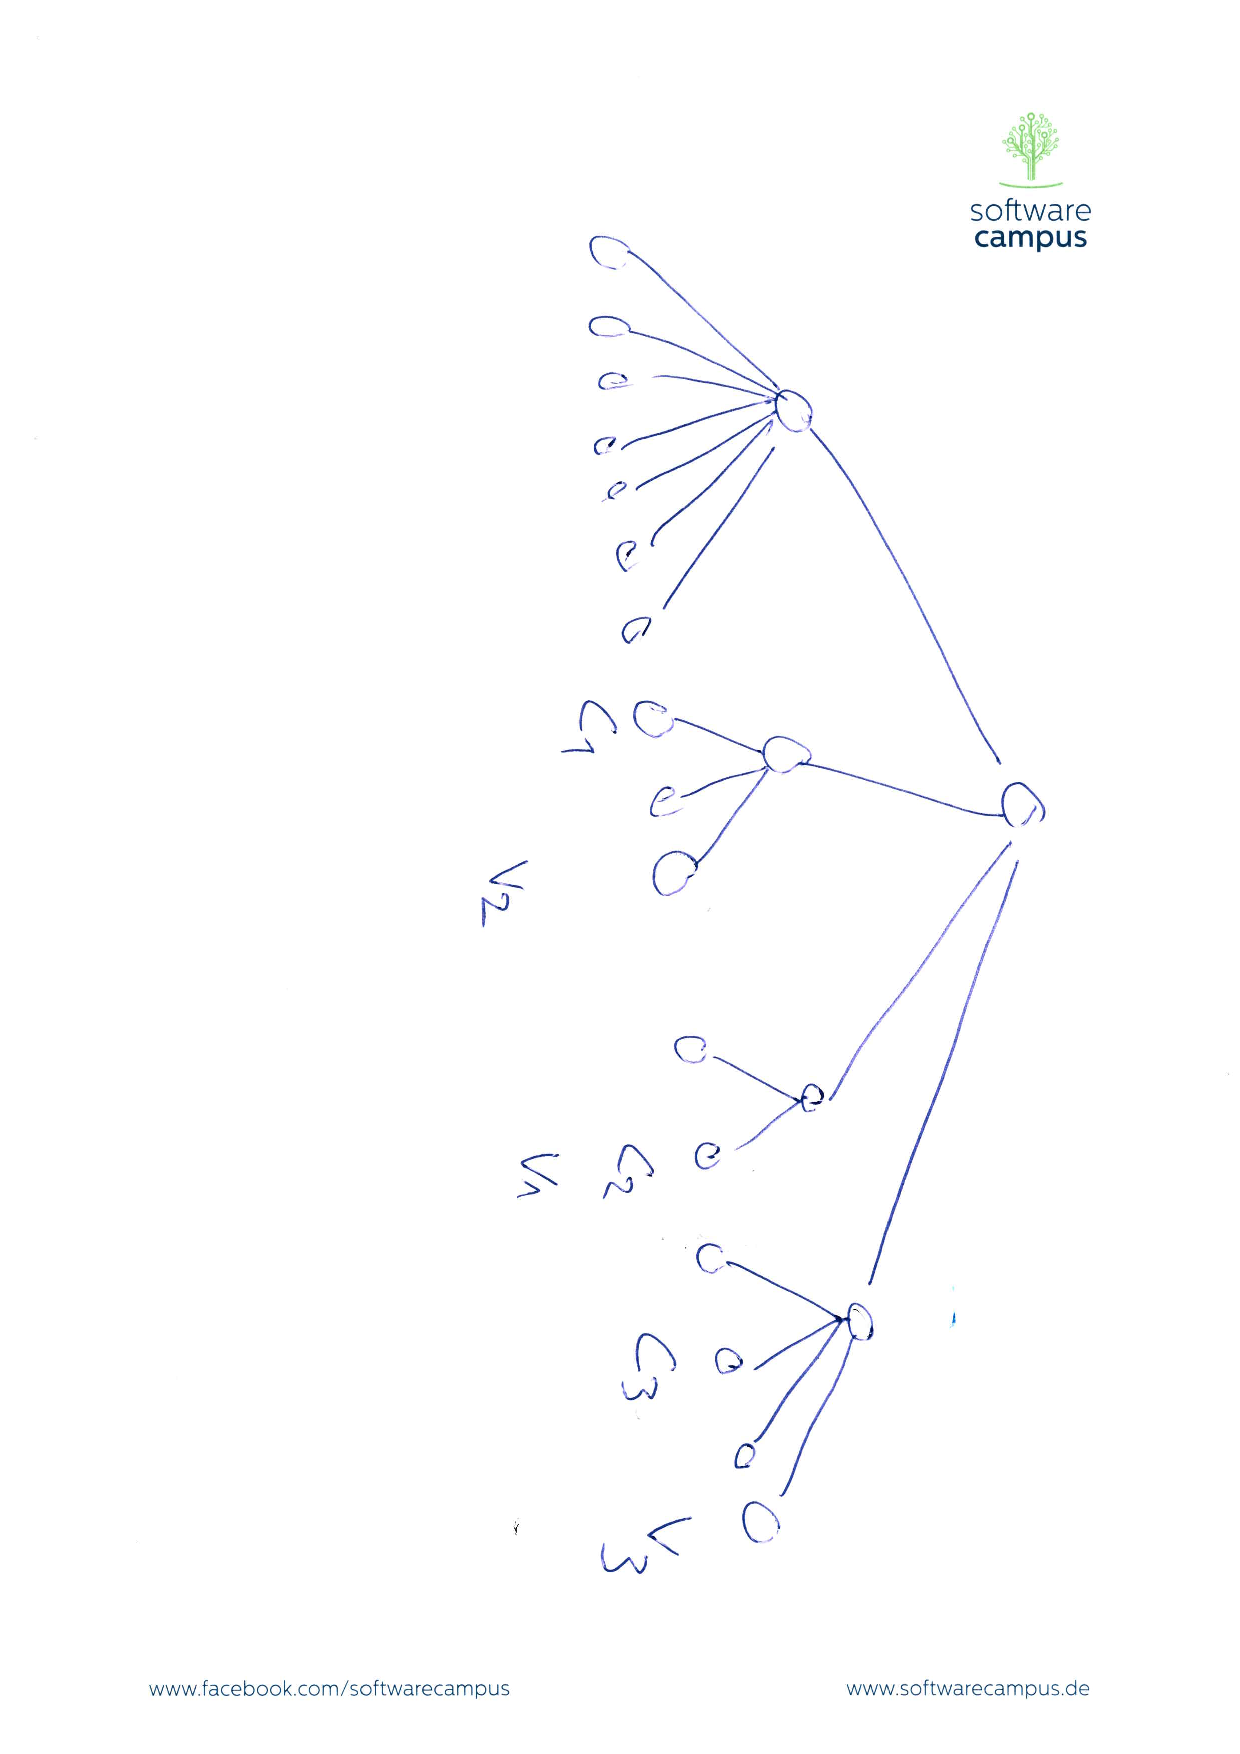
\includegraphics[angle=90,origin=c, height=7cm]{figs/model_fig_skteches/basic_problem}
\caption{basic problem}
\label{fig:basic_problem}
\end{figure}
\begin{figure}

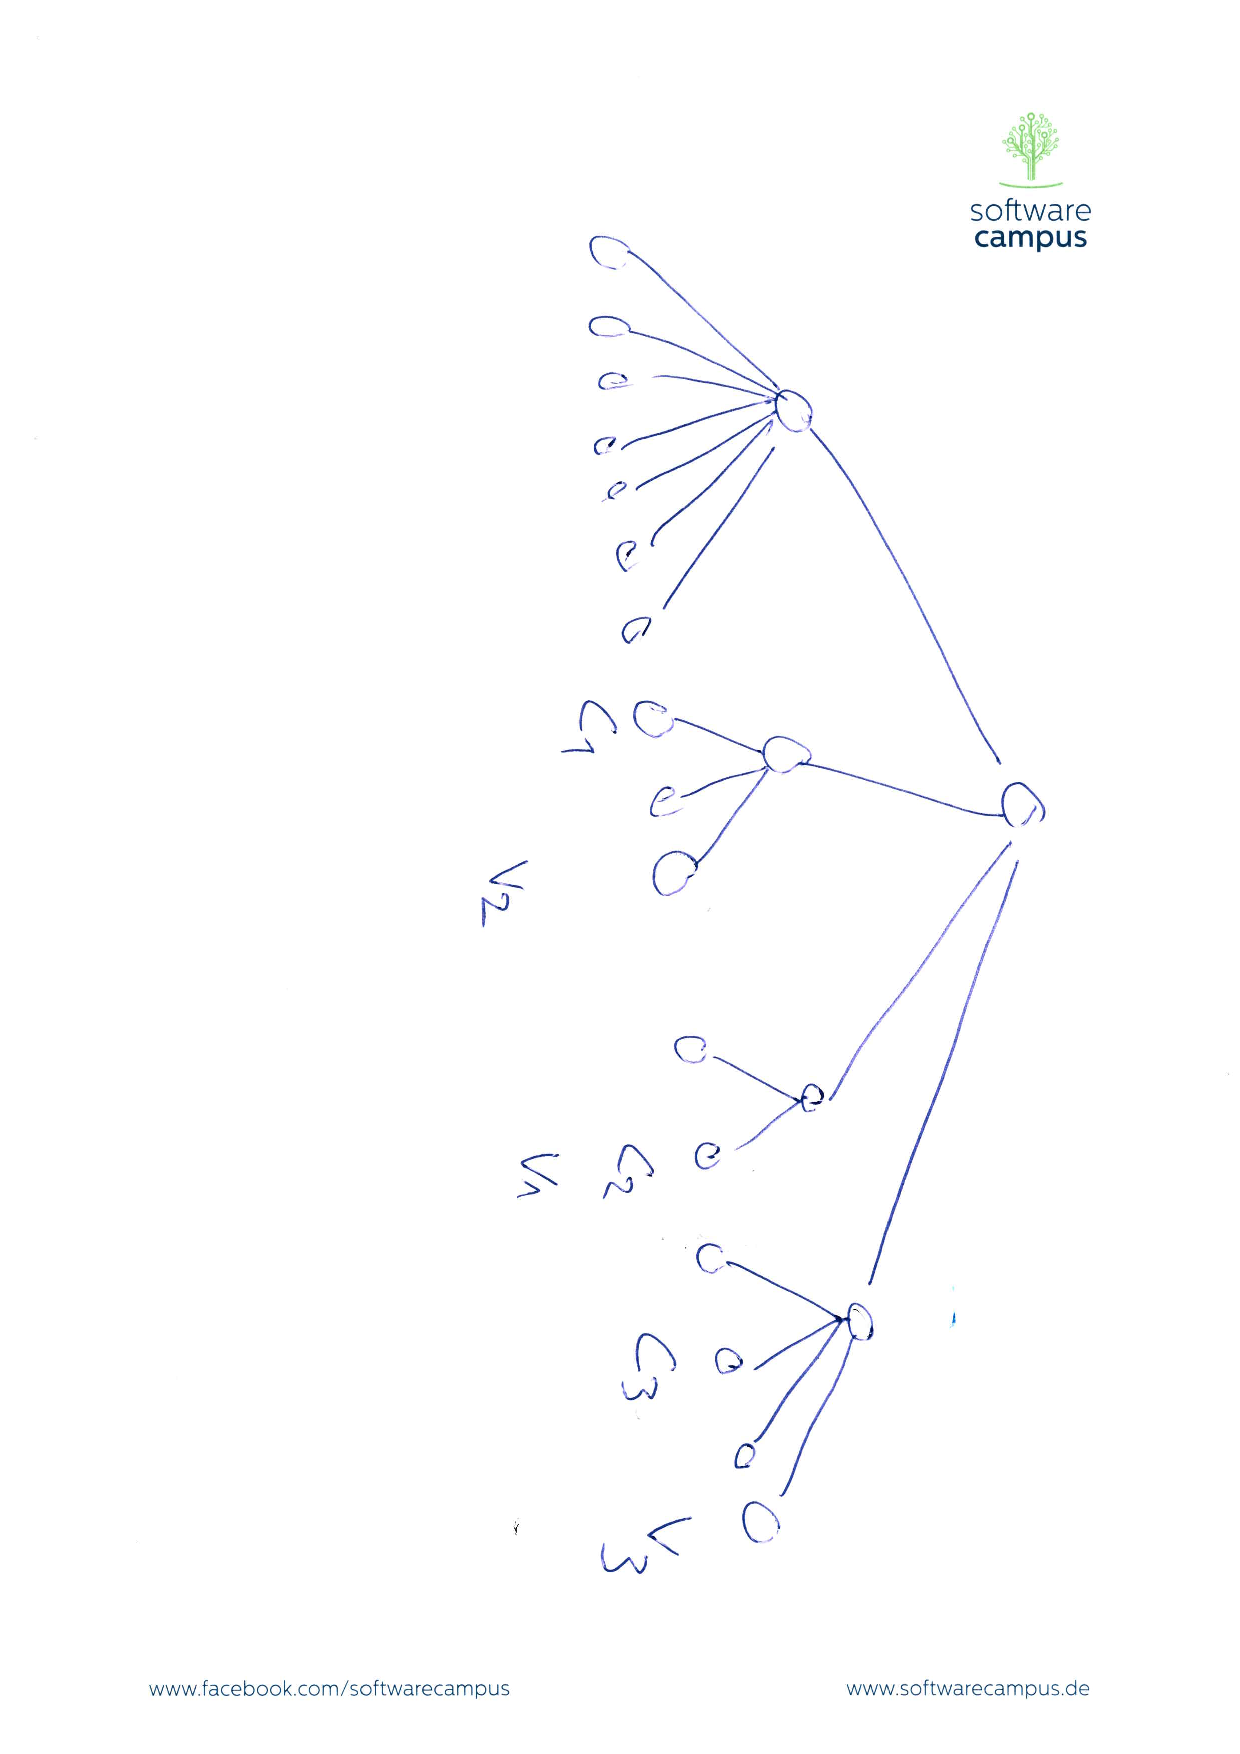
\includegraphics[angle=90,origin=c, height=7cm]{figs/model_fig_skteches/basic_problem}
\caption{solution for basic problem (green is pathes for transfer)}
\end{figure}

Throughout this section we will introduce different properties, to extend this
basic model. These properties can (and will) be combined to form more
challenging instances of $\Problem$.

%\begin{figure}[htbp]
%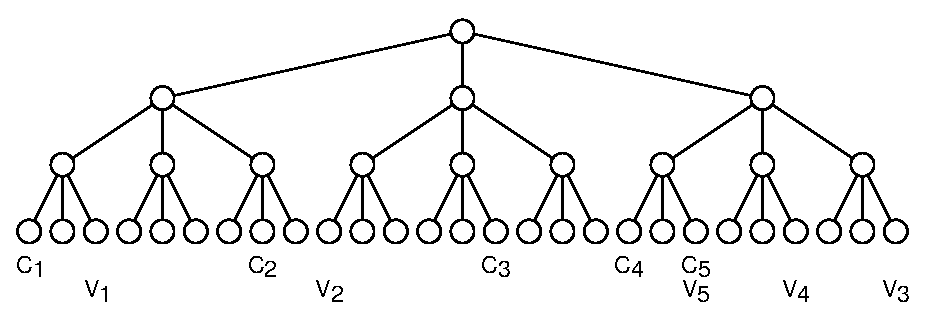
\includegraphics[width = \columnwidth]{figs/basic_scenario_3.eps}
%\caption{An example situation with 5 $\Chunk s$ and $\VM s$. Note that $c_5$
%and $v_5$ are on the same host.}
%\label{fig:model_clean}
%\end{figure}
%
%
%
%Figure~\ref{fig:model_clean} shows an example situation with $n = 5$. The goal
%of the $\Problem$  is to find an assignment of the $\VM s$ to the $\Chunk s$,
%which minimizes the overall bandwidth consumption of the job.
%
%We will now exemplarically examine an assignment of $\Chunk s$ to $\VM s$.
%Assume $c_1$ is assigned to $v_1$, $c2$ to $v2$, $c3$ to $v3$, $c4$ to $v4$
%and $c5$ to $v5$. Since $v_5$ runs on the same host, which contains $c_5$,
%transfering $c_5$ to $v_5$ will consume no bandwidth on the physical links.
%Hence we assume the overall bandwidth costs of the transfer to be $0$. The
%distrance between $v_1$ and $c_1$ is $2$ hops. Hence the transfer of the
%$\Chunk$ to the $\VM$ will consume bandwidth on two links. As a result, the
%overall bandwidth costs is $2 \cdot b_t$, where $b_t$ is the bandwidth
%neccessary for the transfer of a $\Chunk$. $v_4$ is $4$ hops away from $c_4$,
%which results in a total cost of $4 \cdot b_t$. Since the hop distance between
%$v_2$ and $c_2$ is 6, the costs for transferring the $\Chunk$ is $6 \cdot
%b_t$. The same holds for $v_3$ and $c_3$. The overall bandwidth consumption of
%the assignment is hence $18 \cdot b_t$.
%
%This is not an optimal solution for the $\Problem$. To show this, we will
%inspect a similar mapping. The only difference in the optimal mapping, is that
%$v_3$ is assigned to $c_2$ and $v_2$ is assigned to $c_3$. The bandwidth costs
%for transfering $c_2$ to it's assigned $\VM$ do not change, since $v_3$ is
%still $6$ hops away. $c_3$ however is now only $4$ hops away from its assigned
%$\VM$, which results in an overall bandwidth consumption of $16 \cdot b_t$.

\subsection{Communication Costs - $cv$}

\carlo{TODO: new symbol?}

This model extension assumes, that each VM  $\VirtualNode_i \in \VirtualNodes$
has to communicate with each other VM $\VirtualNode_{j \neq i} \in
\VirtualNodes$. Hence, the virtual cluster, which is to be embedded on the
physical substrate no longer consists only of a set of VMs, but is extended by a
set of virtual edges $\VirtualEdges : \VirtualNodes \times \VirtualNodes$.
Similar to the transfer of the chunks to the VMs, these edges have to be mapped
to a path in the host graph, which connects the locations to which the two VMs
are mapped. For the sake of simplicity we assume, that two VMs which communicate
inflict bandwidth cost of $\CostCom$ on each link of the path, which they use
for their communication.

\carlo{NEW: With this model extension the total costs $\Cost = \Cost_T + 
\Cost_C$ are composed of the costs for the transport $\Cost_T$ and the costs 
for communication among the VMs $\Cost_C$. $\Cost_C$ depends only on 
$\NodeMapping$, while $\Cost_T$ depends on $\NodeMapping$ and 
$\VmChunkAssignment$.}

\begin{figure}

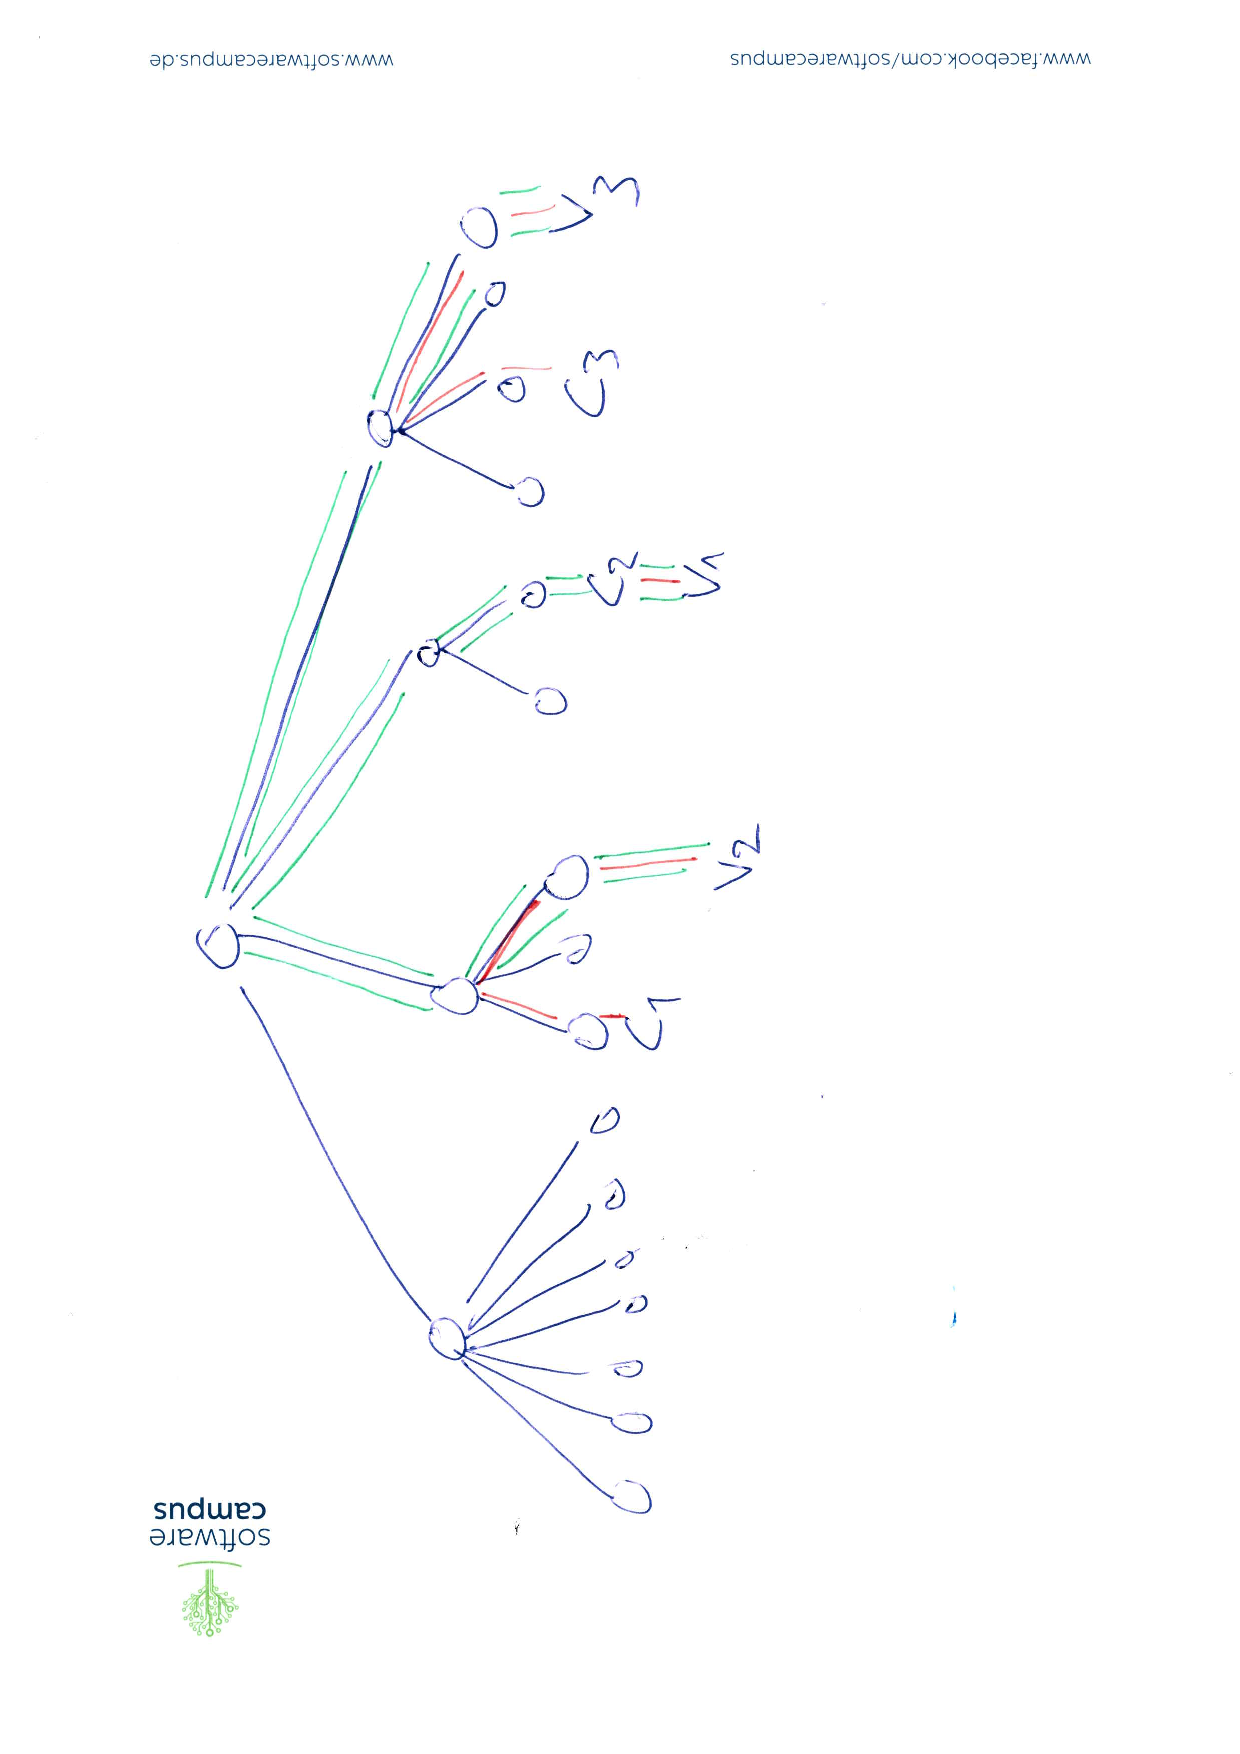
\includegraphics[angle=270,origin=c, height=7cm]{figs/model_fig_skteches/cv}
\caption{solution for problem with cv}
\end{figure}

%So
%far our model accounted bandwidth which is consumed to transfer data from it's
%location in the physical topology to the $\VM$ which will process it. However,
%due to the nature of distributed jobs, the $\VM s$ will also comunicate with
%each other. While we denoted the costs of transfering a chunk over a (1-hop)
%link with $b_t$, we will refer to the bandwidth costs of transfering data
%between a pair of $\VM s$ with $b_c$.


\subsection{Redundant Chunks - $r$}

This property specifies that, instead of having a single chunk $\Chunk_j$, we
have $\RedundancyFactor$ redundant copies of each chunk
$\Chunk_{j_1},\dots,\Chunk_{j_\RedundancyFactor}  \in \Chunks$. These copies are
entirely equal, and only one instance of a specific chunk type (e.g.
$\Chunk_{j_2}$) has to be read by one VM $\VirtualNode_j \in \VirtualNodes$.
Note that we assume chunks to be atomic - they cannot be read from two different
locations, requiering only $\CostTrans / 2$  bandwidth.

\begin{figure}

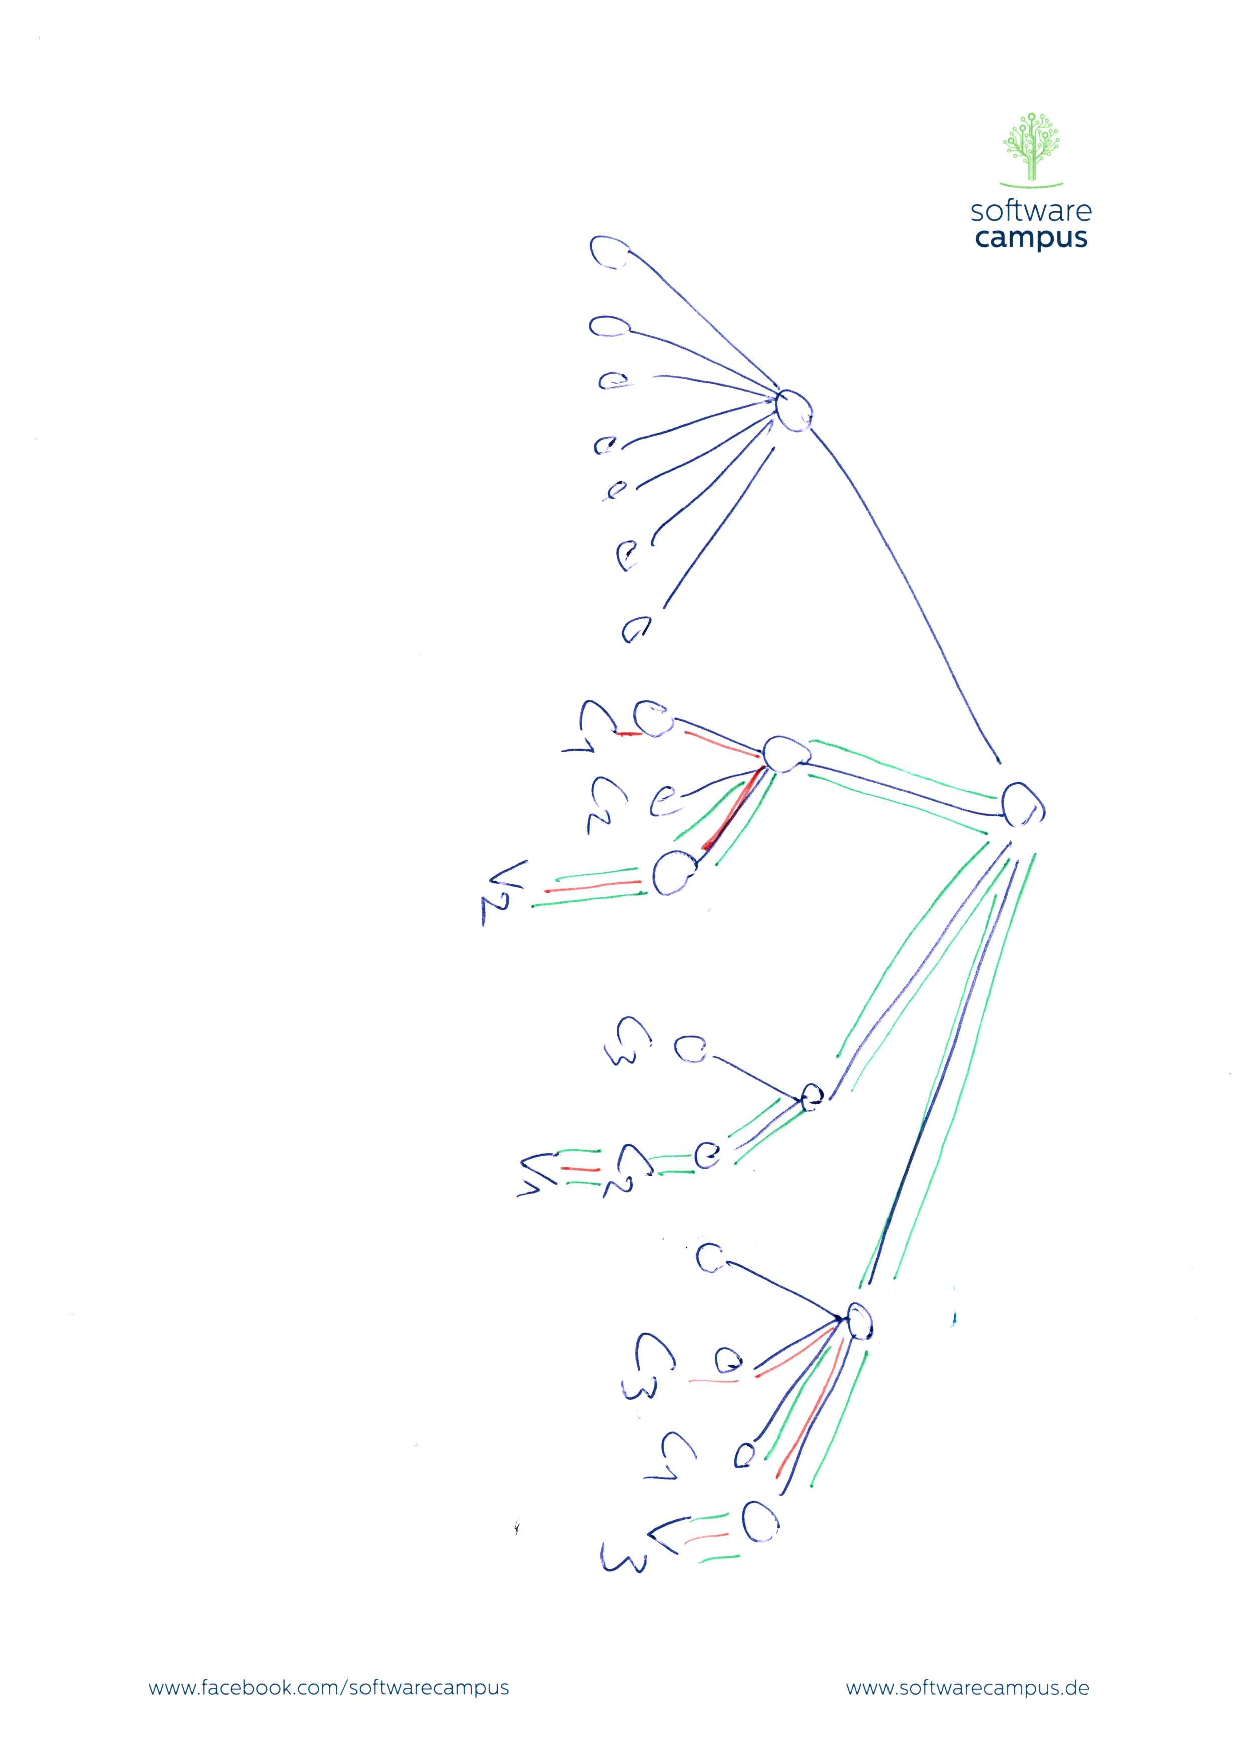
\includegraphics[angle=90,origin=c, height=7cm]{figs/model_fig_skteches/r_cv}
\caption{solution for problem with r}
\end{figure}




\subsection{Multiple Chunks per VM - $ma$}

This extension increases the processing capacities of the VMs. Instead of the
basic 1:1 ratio of VMs and chunks, this extension allows a VM to process
$\MaFactor \in \mathbb{N}^+$ many chunks. We assume, that the data which has to
be transferred to the VM from the chunks cannot be aggregated, and $\Vms =
\ChunkTypes / \MaFactor$.

\begin{figure}

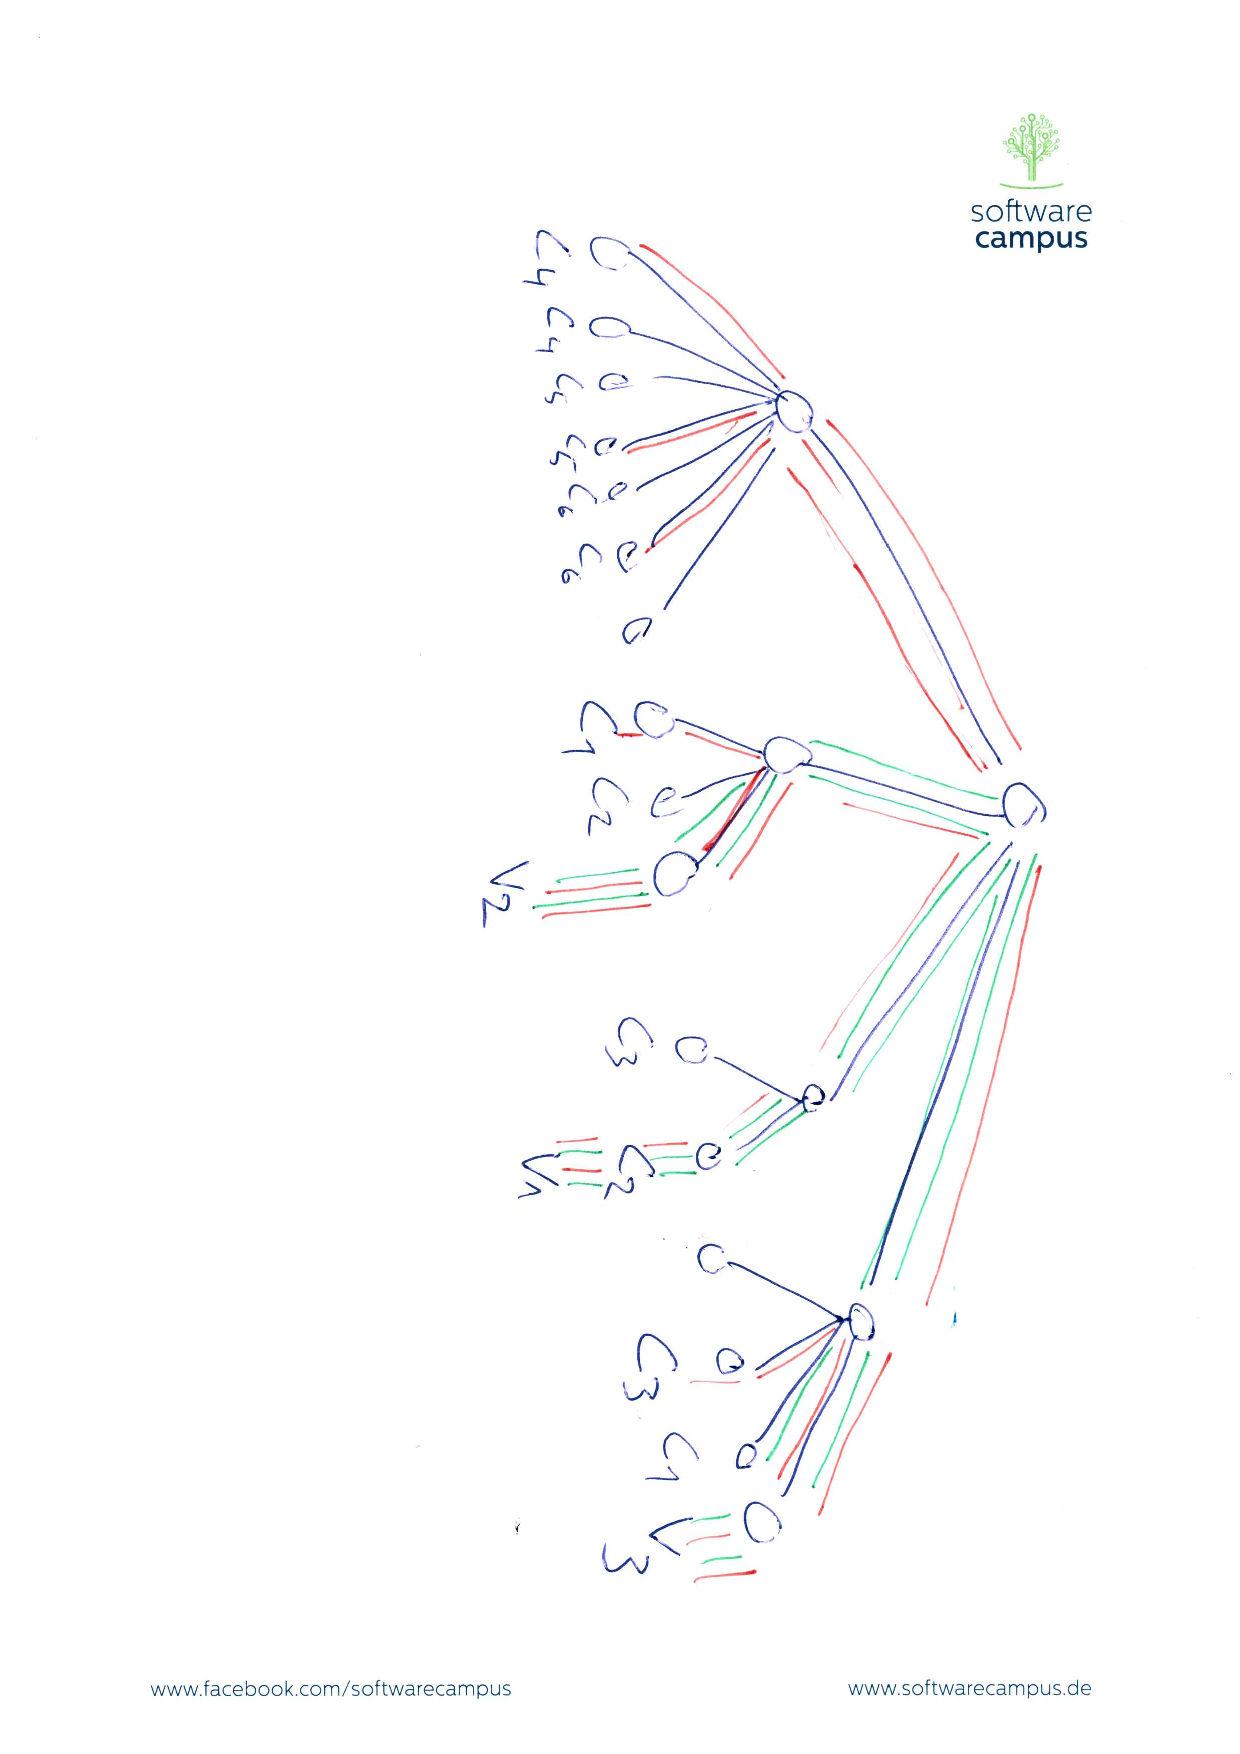
\includegraphics[angle=90,origin=c, height=7cm]{figs/model_fig_skteches/ma_r_cv}
\caption{soltion with ma}
\end{figure}

\subsection{Bandwidth Constraints - $bw$}

So far we only focussed on computing minimal bandwidth costs. However, in
reality the bandwidth which a single link can offer is limited. This model
extension limits the available bandwidth on each link $\SubstrateEdge_i \in
\SubstrateEdges$ in the host graph $\Tree$. We denote the capacity limitations
by $\Capacity : \SubstrateEdges \rightarrow \mathbb{R}$. The sum of all
bandwidth costs on this link, may never exeed it's capacity. Be aware that
this extension introduces infeasible instances.

\begin{figure}

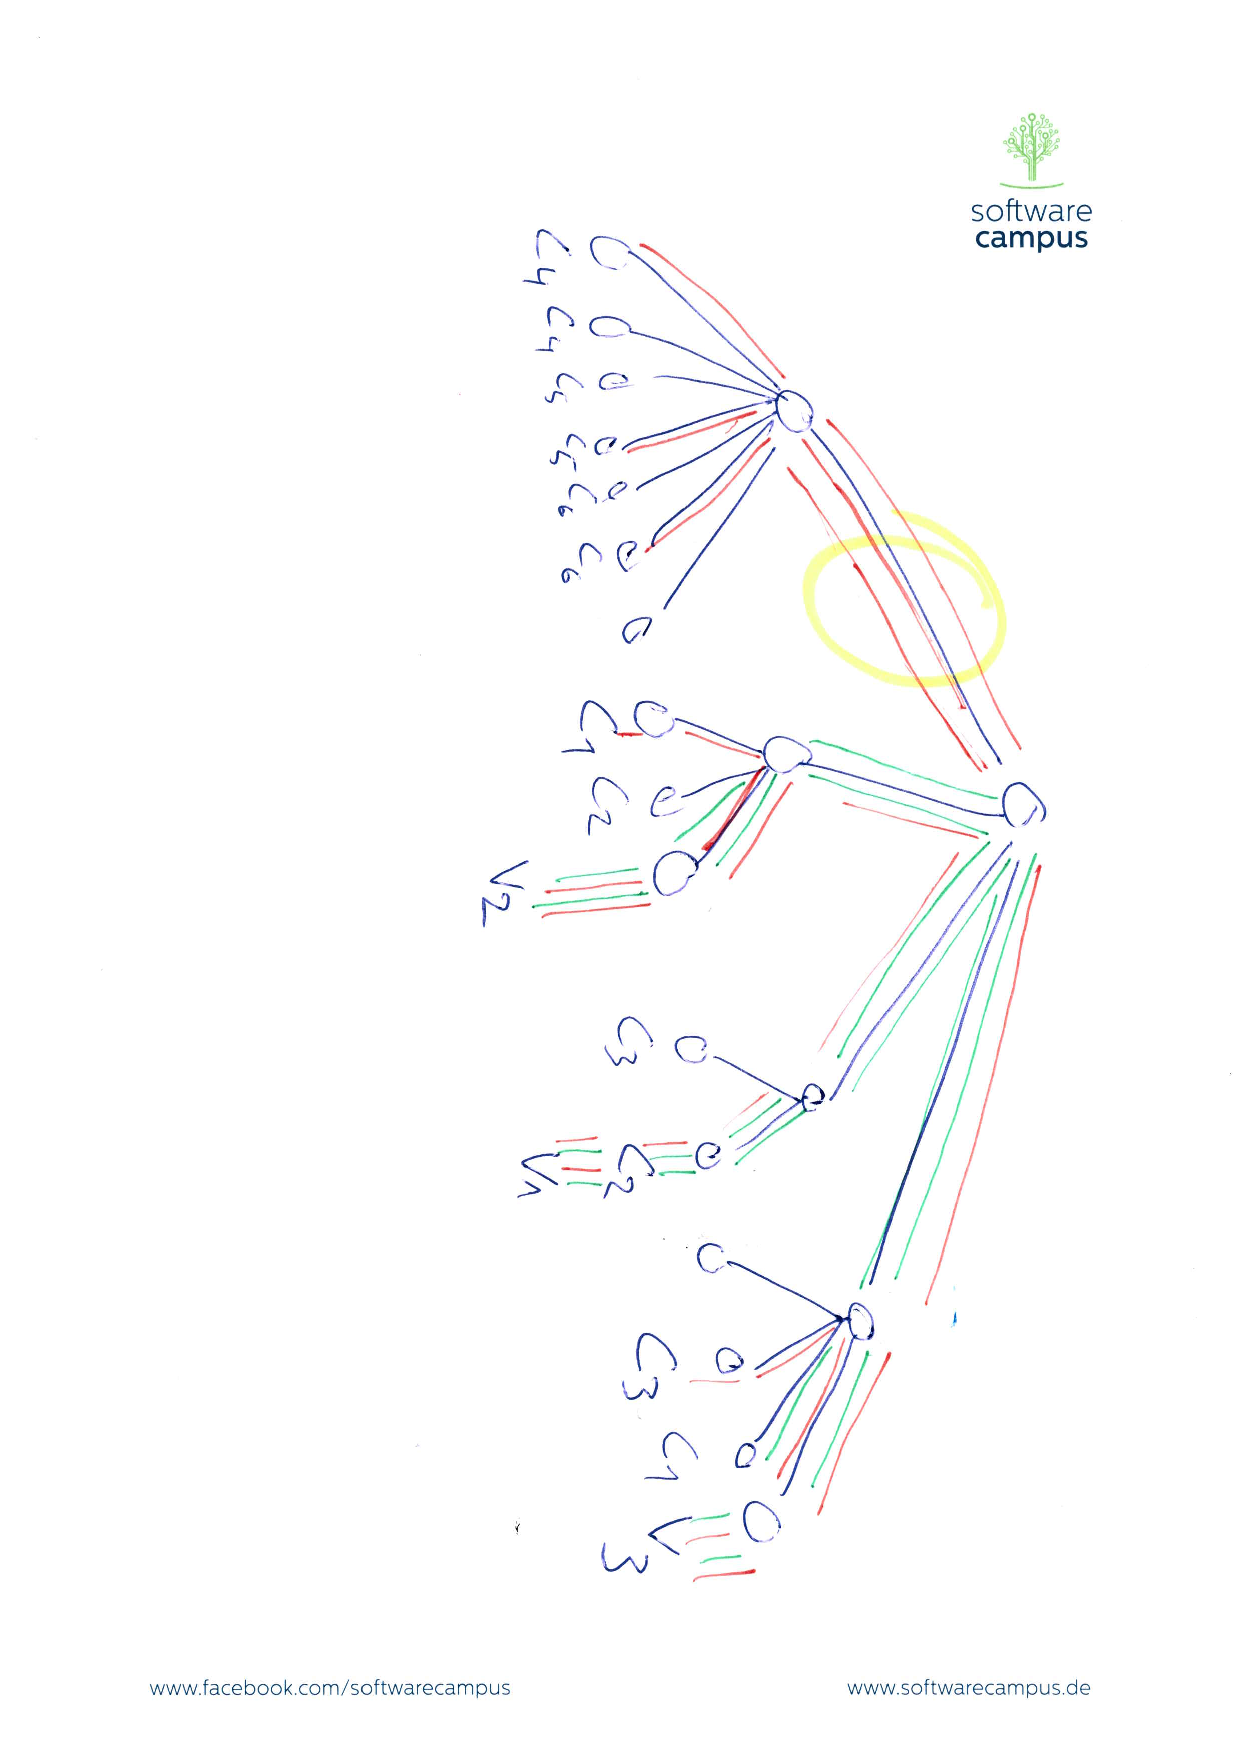
\includegraphics[angle=90,origin=c, height=7cm]{figs/model_fig_skteches/bw_ma_r_cv}
\caption{The bandwidth exceeds the capacity - independent of the chosen assignment}
\end{figure}
\subsection{Free VM Placement - $fp$}

The Free VM Placement property describes a variant of our simple model, where
the positions of the VMs are not given in the problem statement but are
rather chosen by the described strategy. Concretely, $\NodeMapping$ is no
longer given, but part of the optimization within $\Problem$. We assume that
each leaf can only host one VM.

\subsection{Combined models} In this paper we analyse combinations of the 
different properties listed above. 

\begin{figure}[htbp]
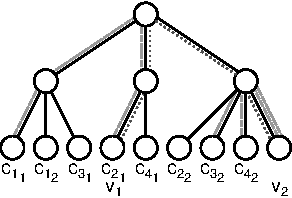
\includegraphics[width =\columnwidth]{figs/model_ma_r_cv}
\caption{An example instance of $\Problem$ with $ma$ + $cv$ + $r$. An
optimal solution is indicated by the dashed (transport costs) and dotted 
(communication costs) lines. }
\label{fig:model_combined}
\end{figure}

An example of this can be seen in Figure~\ref{fig:model_combined}, which shows 
an instance of $\Problem$, with the additional properties $ma$, $cv$ and $r$. 
The host graph consists of 14 nodes. 9 nodes are leaves; 2 VMs are allready 
embedded on leaves; with $\RedundancyFactor = 2$ and $\MaFactor = 2$ we have 4 
chunk types, and two VMs of each type. The solution to this instance is also 
depicted: The data from $\Chunk_{1_1}$ and $\Chunk_{2_1}$ is read by 
$\VirtualNode_1$, $\Chunk_{3_2}$ and $\Chunk_{4_2}$ are read by 
$\VirtualNode_2$. The dashed light gray lines indicate transport 
costs $\CostTrans$. Note that no bandwidth is neccessary to transport data from 
$\Chunk_{2_1}$ to $\VirtualNode_1$, since these are collocated. The link 
connecting the node, which hosts $\VirtualNode_2$ with it's parent, the 
transport costs ammount to $2 \CostTrans$ - indicated by two dashed lines. In 
addition to this, the figure illustrates the communication costs $\CostCom$, 
which are indicated by the dotted dark gray line.

%\subsection{Summary of our results}

\begin{figure}[htbp]
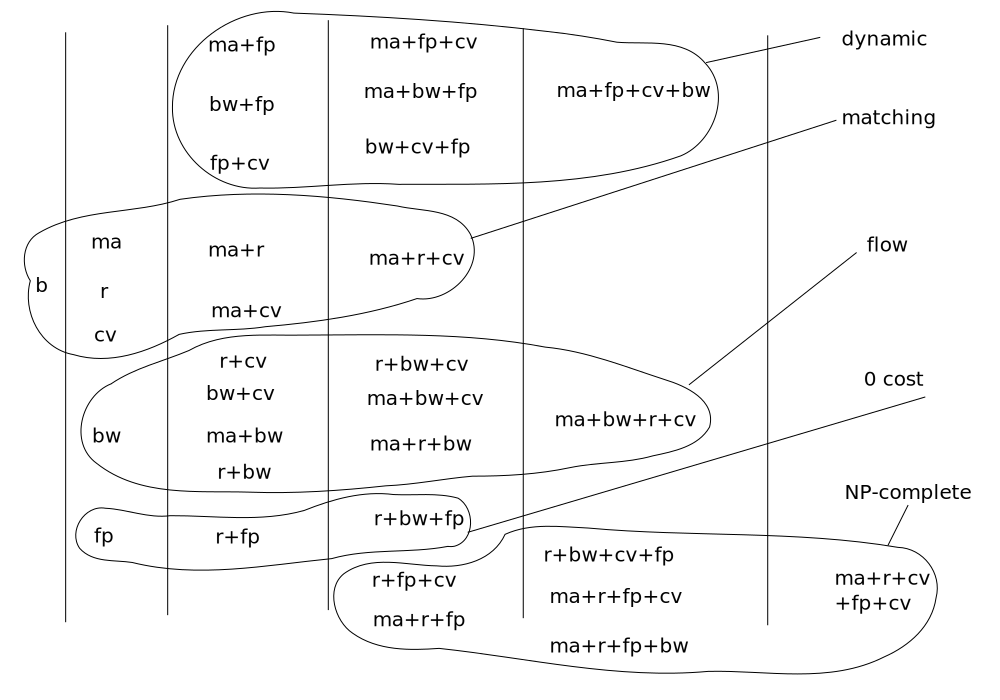
\includegraphics[width = \columnwidth]{figs/summary}
\caption{foo}
\label{fig:summary}
\end{figure}

This paper presents polynomial time algorithms or NP-hardness prooves for 
\textit{all} possible comibnations of properties. An overview, of which problem 
can be solved by which algorihms can be found in Figure~\ref{fig:summary}.

\begin{comment}
\begin{enumerate}
\item basic problem - M
\item ma - M
\item r - M
\item cv - reduces to basic problem
\item bw - F
\item fp - solution of 0 cost
\item ma + r - M
\item  ma + bw - F
\item ma + cv - reduces to ma
\item ma + fp - D
\item r + bw - F
\item r + cv - reduces to r
\item r + fp - solution of 0 cost
\item bw + cv - reduces to bw
\item bw + fp - D
\item fp + cv - D
\item ma + r + bw - F
\item ma + r + cv - reduces to ma + r
\item ma + r + fp - N
\item ma + bw + cv - reduces to ma + bw
\item ma + bw + fp - D
\item ma + fp + cv - D
\item r + bw + cv - reduces to r + bw
\item r + cv + fp - N
\item r + bw + fp - solution of 0 cost
\item bw + cv + fp - D
\item ma + r + bw + cv - reduces to ma + r + bw
\item ma + r + bw + fp - N
\item ma + r + cv + fp - N
\item ma + fp + cv + bw - D
\item r + bw + cv + fp - N
\item ma + r + bw + cv + fp - N
\end{enumerate}
\end{comment}




